% Created 2016-01-17 Sun 20:47
\documentclass[11pt]{article}
\usepackage[utf8]{inputenc}
\usepackage{lmodern}
\usepackage[T1]{fontenc}
\usepackage{fixltx2e}
\usepackage{graphicx}
\usepackage{longtable}
\usepackage{float}
\usepackage{wrapfig}
\usepackage{rotating}
\usepackage[normalem]{ulem}
\usepackage{amsmath}
\usepackage{textcomp}
\usepackage{marvosym}
\usepackage{wasysym}
\usepackage{amssymb}
\usepackage{amsmath}
\usepackage[version=3]{mhchem}
\usepackage[numbers,super,sort&compress]{natbib}
\usepackage{natmove}
\usepackage{url}
\usepackage{minted}
\usepackage{underscore}
\usepackage[linktocpage,pdfstartview=FitH,colorlinks,
linkcolor=blue,anchorcolor=blue,
citecolor=blue,filecolor=blue,menucolor=blue,urlcolor=blue]{hyperref}
\usepackage{attachfile}
\usepackage{graphicx}
\usepackage{subfigure}
\usepackage{pdfcomment}
\date{\today}
\title{blog}
\begin{document}

\section{{\bfseries\sffamily TODO} Side by side figures in org-mode for different outputs}
\label{sec-1}
Occasionally, someone wants side by side figures with subcaptions that have individually referenceable labels. This is not too hard in \LaTeX{}, and there is a solution here:  \url{http://www.johndcook.com/blog/2009/01/14/how-to-display-side-by-side-figurs-in-latex/}.

We can create side by side figures in raw \LaTeX{} like this (note however, this will not show up in html export):

\begin{figure}
  \subfigure[Left graph \label{fig:a}]
    {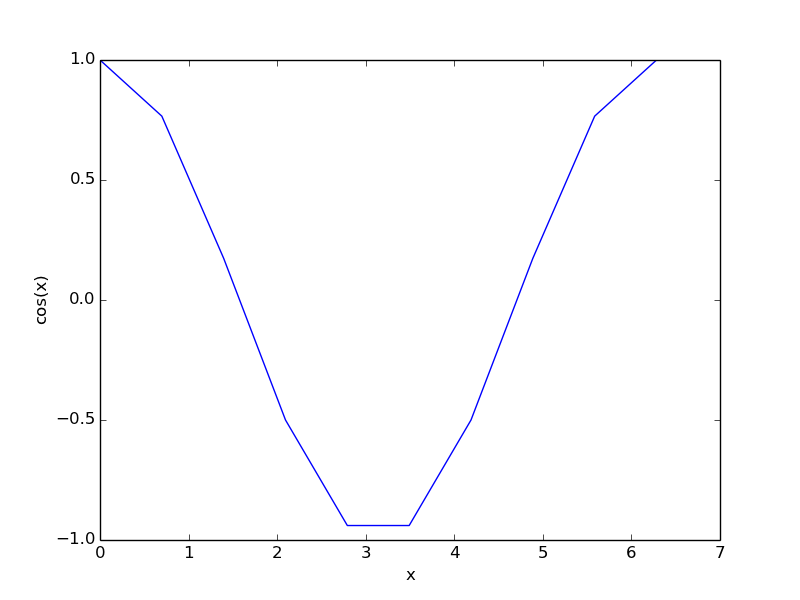
\includegraphics[width=3in]{images/cos-plot.png}}
\enskip % horizontal spacking. tex.stackexchange.com/questions/41476/lengths-and-when-to-use-them
  \subfigure[Right graph. \label{fig:b}]
    {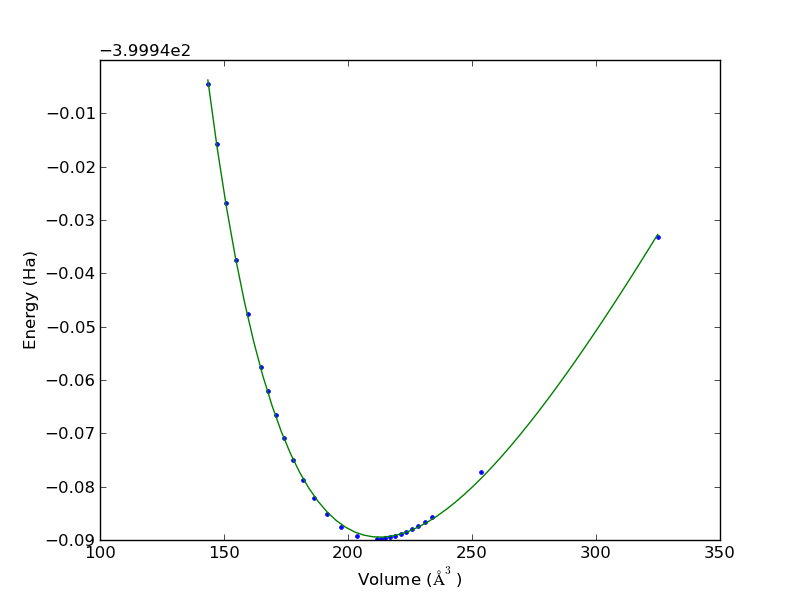
\includegraphics[width=3in]{images/eos-uncertainty.png}}
\caption{Text pertaining to both graphs,\ref{fig:a}and \ref{fig:b}. \label{fig12}}
\end{figure}

And in our text we can refer to the overall Figure \ref{fig12}, or the subfigures Figure \ref{fig:a} or Figure \ref{fig:b}. This works fine if your end goal is \LaTeX{} export. It does not work fine if you want to consider HTML or some other output.

So, here we consider how we could remove the \LaTeX{} dependency by representing the figures in a sexp data structure, for example something like this. I change the labels and captions a bit so they are actually distinguishable.

\begin{minted}[frame=lines,fontsize=\scriptsize,linenos]{common-lisp}
(figure ()
 (subfigure '("Left graph from sexp." (label "fig:sa"))
            (includegraphics '((width . "3in"))
                             "images/cos-plot.png"))
 (enskip)
 (subfigure '("Right graph from sexp" (label "fig:sb"))
            (includegraphics '((width . "3in"))
                             "images/eos-uncertainty.png"))
 (caption
  "Text pertaining to both graphs from a sexp, " (ref "fig:sa")
  " and " (ref "fig:sb") "." (label "figs12")))
\end{minted}

\begin{verbatim}
"emacs-lisp"
\end{verbatim}

This doesn't look much worse than the \LaTeX{} code itself. It might not seem useful right away, but imagine if this was really code that could evaluate to the format we want. Remember the \href{http://kitchingroup.cheme.cmu.edu/blog/2015/06/10/A-sexp-version-of-a-bibtex-entry/}{sexp bibtex entry} that could evaluate to bibtex, json or xml? Let's look at this here. What we consider is kind of like \url{http://oremacs.com/2015/01/23/eltex/}, but we could include other kinds of exports if we wanted.

Here is our special block in org-mode. It should render roughly as side by side images in \LaTeX{} and HTML.

\begin{figure}
\subfigure[Left graph from sexp.\label{fig:sa}]{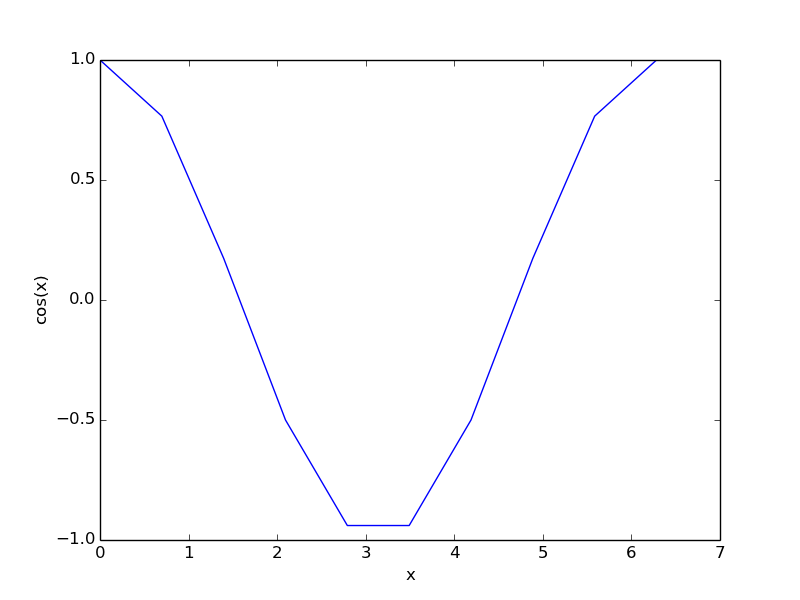
\includegraphics[width=3in]{images/cos-plot.png}}
\enskip
\subfigure[Right graph from sexp\label{fig:sb}]{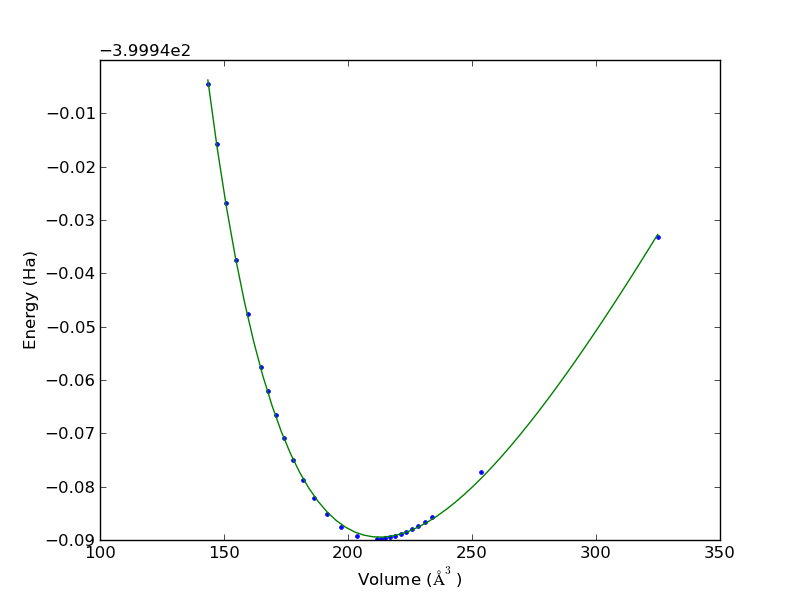
\includegraphics[width=3in]{images/eos-uncertainty.png}}
\caption{Text pertaining to both graphs from a sexp, \ref{fig:sa} and \ref{fig:sb}.\label{figs12}}
\end{figure}

Now, we need a function to format the sexp block for export. It is easy, we just eval the contents of the block. We do assume here there is just one sexp to evaluate. This function will handle all special blocks, but we only want to do something different for the sexp blocks.

\begin{minted}[frame=lines,fontsize=\scriptsize,linenos]{common-lisp}
(defun sb-format (sb contents info)
  (cond
     ((string= "SEXP" (org-element-property :type sb))
      (eval (read (buffer-substring
                   (org-element-property :contents-begin sb)
                   (org-element-property :contents-end sb)))))
     (t
      contents)))))
\end{minted}

\begin{verbatim}
sb-format
\end{verbatim}

All that is left is to define the functions. We do that next.

\subsection{Latex export}
\label{sec-1-1}

We need to define a function for each piece of the data structure that will evaluate to a string. Here are three easy ones.

\begin{minted}[frame=lines,fontsize=\scriptsize,linenos]{common-lisp}
(defun label (arg)
  (format "\\label{%s}" arg))

(defun ref (arg)
  (format "\\ref{%s}" arg))

(defun caption (&rest body)
  (format "\\caption{%s}"
         (mapconcat 'eval body "")))

(caption
  "Text pertaining to both graphs, " (ref "fig:a")
  " and " (ref "fig:b") "." (label "fig12"))
\end{minted}
\begin{verbatim}
\caption{Text pertaining to both graphs, \ref{fig:a} and \ref{fig:b}.\label{fig12}}
\end{verbatim}

Now, for includegraphics, we allow options and a path. The options we assume are in an a-list.

\begin{minted}[frame=lines,fontsize=\scriptsize,linenos]{common-lisp}
(defun includegraphics (options path)
  (format "\\includegraphics%s{%s}"
          (if options
              (format "[%s]"
                      (mapconcat (lambda (ccell)
                                   (format "%s=%s"
                                           (car ccell)
                                           (cdr ccell)))
                                 options
                                 ","))
            "")
          path))

(includegraphics '((width . "3in"))
                 "images/eos-uncertainty.png")
\end{minted}
\begin{verbatim}
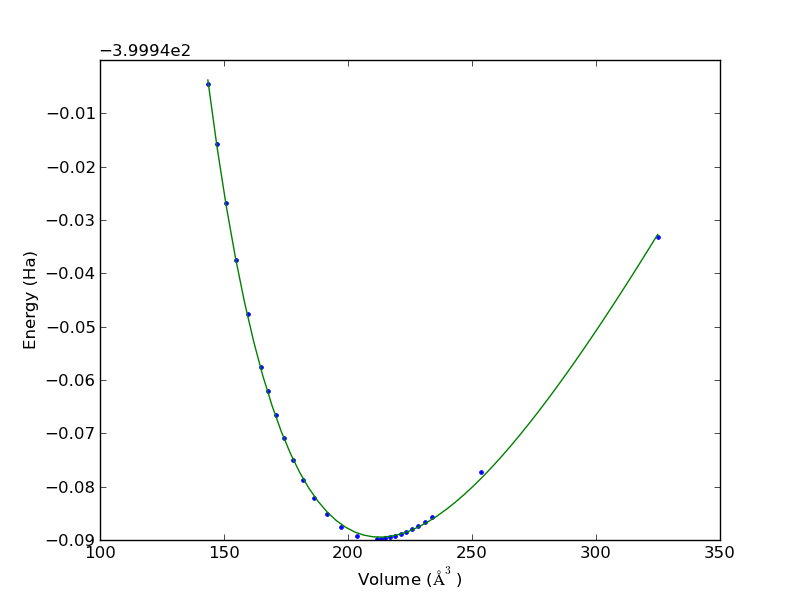
\includegraphics[width=3in]{images/eos-uncertainty.png}
\end{verbatim}

Similarly for subfigure, we have options, and then a body of expressions. The options here are just expressions that should evaluate to strings. This is not consistent with the way we do options in includegraphics. This is just proof of concept work, so I don't know if this inconsistency is really problematic yet, or insufficient for all options.

\begin{minted}[frame=lines,fontsize=\scriptsize,linenos]{common-lisp}
(defun subfigure (options &rest body)
  (format "\\subfigure%s{%s}"
          (if options
              (format "[%s]"
                      (mapconcat 'eval options ""))
            "")
          (mapconcat 'eval body "")))

(subfigure '("Right graph" (label "fig:b"))
            (includegraphics '((width . "3in"))
                             "images/eos-uncertainty.png"))
\end{minted}
\begin{verbatim}
\subfigure[Right graph\label{fig:b}]{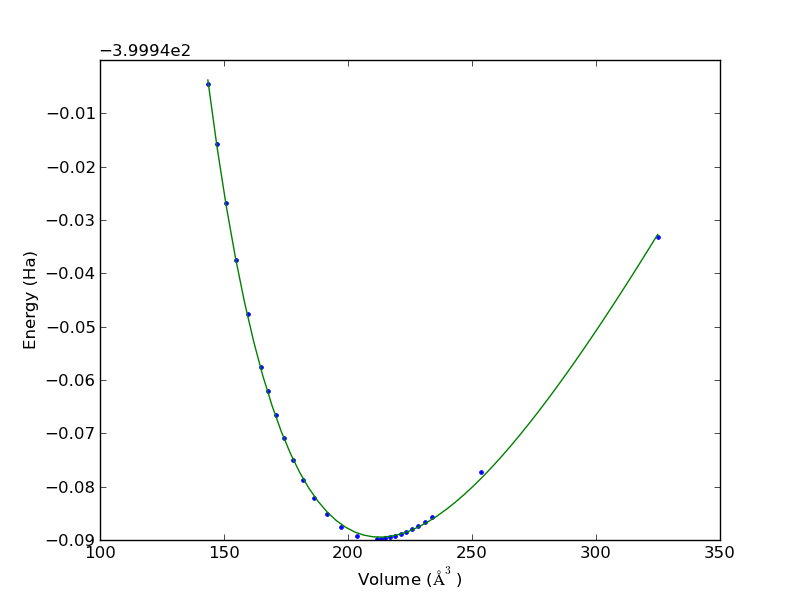
\includegraphics[width=3in]{images/eos-uncertainty.png}}
\end{verbatim}

Now, we put the whole figure together.

\begin{minted}[frame=lines,fontsize=\scriptsize,linenos]{common-lisp}
(defun figure (options &rest body)
  (format "\\begin{figure}
%s
\\end{figure}"
(mapconcat 'eval body "\n")))

(defun enskip () "\\enskip")
\end{minted}
\begin{verbatim}
enskip
\end{verbatim}

Now, we would have a block like this, and we can evaluate it.

\begin{minted}[frame=lines,fontsize=\scriptsize,linenos]{common-lisp}
(figure ()
 (subfigure '("Left graph from sexp." (label "fig:ssa"))
            (includegraphics '((width . "3in"))
                             "images/cos-plot.png"))
 (enskip)
 (subfigure '("Right graph from sexp" (label "fig:ssb"))
            (includegraphics '((width . "3in"))
                             "images/eos-uncertainty.png"))
 (caption
  "Text pertaining to both graphs from a sexp, " (ref "fig:ssa")
  " and " (ref "fig:ssb") "." (label "figss12")))
\end{minted}

\begin{figure}
\subfigure[Left graph from sexp.\label{fig:ssa}]{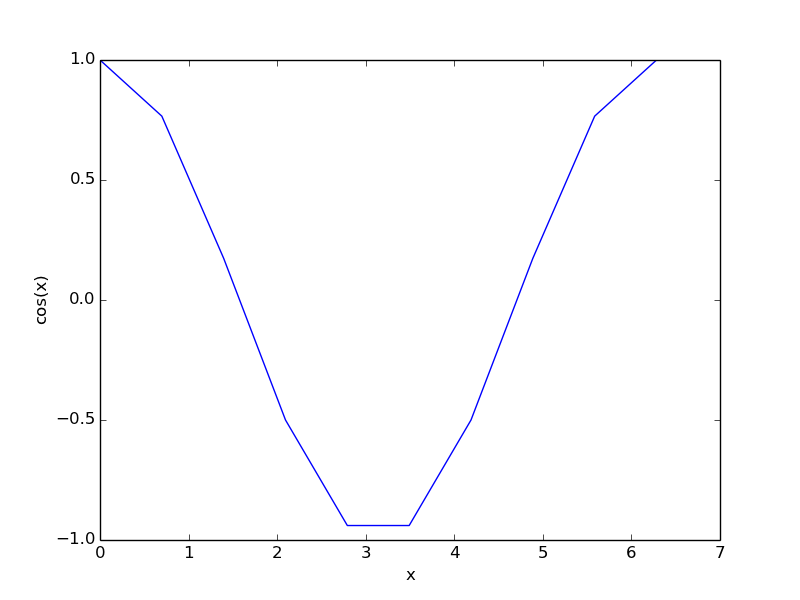
\includegraphics[width=3in]{images/cos-plot.png}}
\enskip
\subfigure[Right graph from sexp\label{fig:ssb}]{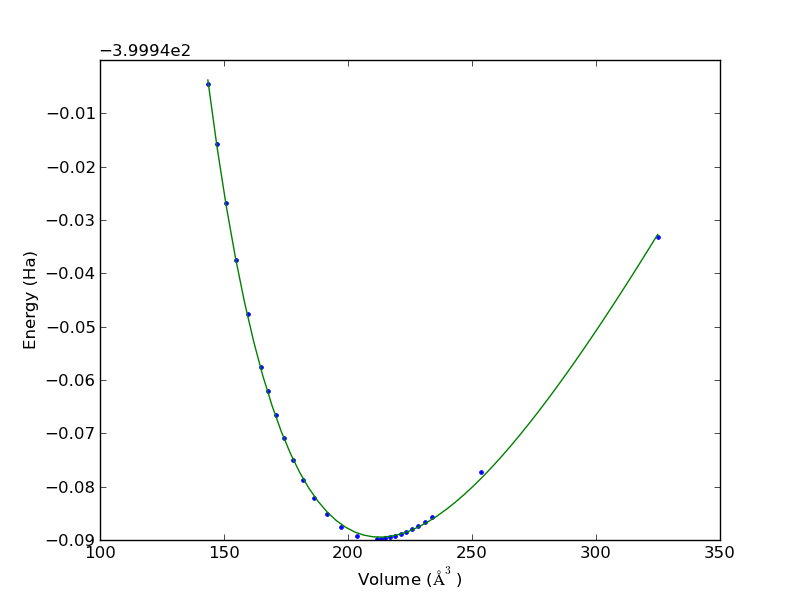
\includegraphics[width=3in]{images/eos-uncertainty.png}}
\caption{Text pertaining to both graphs from a sexp, \ref{fig:ssa} and \ref{fig:ssb}.\label{figss12}}
\end{figure}

Not the most beautiful \LaTeX{} ever, but it works. Now, to get this to work, we need to handle our special sexp blocks differently. We do that with a new derived backend.

\begin{minted}[frame=lines,fontsize=\scriptsize,linenos]{common-lisp}
(org-export-define-derived-backend 'my-latex 'latex
  :translate-alist '((special-block . sb-format)))

(org-latex-compile (org-export-to-file 'my-latex "custom-sb-export.tex"))
(org-open-file "custom-sb-export.pdf")
\end{minted}

\subsection{HTML functions}
\label{sec-1-2}
We need to define each element and its HTML output.
\begin{minted}[frame=lines,fontsize=\scriptsize,linenos]{common-lisp}
(defun label (arg)
  (format "<a name=\"%s\"></a>" arg))

(defun ref (arg)
  (format "<a href=\"#%s\">%s</a>" arg arg))

(defun caption (&rest body)
  (format "<caption>%s</caption>"
         (mapconcat 'eval body "")))

(caption
  "Text pertaining to both graphs, " (ref "fig:a")
  " and " (ref "fig:b") "." (label "fig12"))
\end{minted}

\begin{verbatim}
<caption>Text pertaining to both graphs, <a href="#fig:a">fig:a</a> and <a href="#fig:b">fig:b</a>.<a name="fig12"></a></caption>
\end{verbatim}


We will ignore options for the includegraphics html output. We would need to specify some way to do unit conversions for html. Here we fix the width.
\begin{minted}[frame=lines,fontsize=\scriptsize,linenos]{common-lisp}
(defun includegraphics (options path)
  (format "<img src=\"%s\" width=\"300\">"
          path))

(includegraphics '((width . "3in"))
                 "images/eos-uncertainty.png")
\end{minted}

\begin{verbatim}
<img src="images/eos-uncertainty.png" width="300">
\end{verbatim}

We wrap a subfigure in a table cell.
\begin{minted}[frame=lines,fontsize=\scriptsize,linenos]{common-lisp}
(defun subfigure (options &rest body)
  (format "<td>%s%s</td>"
          (mapconcat 'eval body "")
          (when options
            (concat "<br>"
                    (mapconcat 'eval options "")))))

(subfigure '("Right graph" (label "fig:b"))
            (includegraphics '((width . "3in"))
                             "images/eos-uncertainty.png"))
\end{minted}

\begin{verbatim}
<td><img src="images/eos-uncertainty.png" width="200"><br>Right graph<a name="fig:b"></a></td>
\end{verbatim}

We assume we can put the images in a single row.

\begin{minted}[frame=lines,fontsize=\scriptsize,linenos]{common-lisp}
(defun figure (options &rest body)
  (format "<span class=\"image\"><table>
<tr>%s</tr>
</table></span>"
(mapconcat 'eval body "\n")))

(defun enskip () "")
\end{minted}

\begin{verbatim}
enskip
\end{verbatim}

Now, here is our specification.
\begin{minted}[frame=lines,fontsize=\scriptsize,linenos]{common-lisp}
(figure ()
 (subfigure '("Left graph" (label "fig:a"))
            (includegraphics '((width . "3in"))
                             "images/cos-plot.png"))
 (enskip)
 (subfigure '("Right graph" (label "fig:b"))
            (includegraphics '((width . "3in"))
                             "images/eos-uncertainty.png"))
 (caption
  "Text pertaining to both graphs, " (ref "fig:a")
  " and " (ref "fig:b") "." (label "fig12")))
\end{minted}

And our derived backend for HTML.
\begin{minted}[frame=lines,fontsize=\scriptsize,linenos]{common-lisp}
(org-export-define-derived-backend 'my-html 'html
  :translate-alist '((special-block . sb-format)))

(browse-url (org-export-to-file 'my-html "custom-sb-export.html"))
\end{minted}

\begin{verbatim}
#<process open custom-sb-export.html>
\end{verbatim}

\subsection{Summary thoughts}
\label{sec-1-3}
I think I like the idea. Obviously there are differences between what is possible between \LaTeX{} and HTML, notably the attributes that may or may not be supported between them, including the units of the width, labels, and references. I still have not figured out an elegant way to switch between \LaTeX{} and HTML exports since there is basically one set of functions that need different outputs under different conditions.

For small things, you could achieve this with inline emacs-lisp src blocks, but I think those are limited to one liners. Alternatively, you could probably get by with output from an actual src block, but you would have to make sure it executed during export (I turn this off by default).
% Emacs 25.0.50.1 (Org mode 8.2.10)
\end{document}